\section{\texttt{modal}}\label{sec:example_modal}


This example presents a combination of two statistical inverse problems in one. 
It presents the capability of the Multilevel method in sampling from a target distribution that has either one or two models. The random variable of interest has three parameters, i.e., $\bv{\theta}=(\theta_1,\theta_2, \sigma^2) \in \mathbb{R}^3$, where the third parameter may be seen as variation.

The example also it gives the user the opportunity to chose either one single type of prior distribution, uniform, for the three components of the random variable, or two different priors: a uniform and a beta distribution.

Choosing between a one-mode or a two-mode target distribution is done at execution level, as presented in the following code line:

\begin{lstlisting}[label={},caption={}]
$ cd $HOME/LIBRARIES/QUESO-0.50.0/
$ cd examples/modal
$ rm outputData/*
$ ./modal_gsl example.inp <num_of_nodes>
\end{lstlisting}
where \verb+<num_of_nodes>+ is either 1 or 2.
% 
% 
% This simple statistical inverse problem presents a combination of two, suppose a random variable of interest with three parameters $\bv{\theta}=(\theta_1,\theta_2, \sigma) \in \mathbb{R}^3$,  namely $\bv{\theta}:[0,3]\times[0,3]\times[0,0.3] \rightarrow\mathbb{R}$. 
% 
% 
% 
% This simple statistical inverse problem, suppose a random variable of interest with three parameters $\bv{\theta}=(\theta_1,\theta_2, \sigma) \in \mathbb{R}^3$,  namely $\bv{\theta}:[0,3]\times[0,3]\times[0,0.3] \rightarrow\mathbb{R}$. 
% 
% 
% Suppose also that the distribution we aim to sample has either one or two modes.
% 
\subsection{One-mode distribution}

In this case, the target distribution is assumed to have only one mode.
Suppose also that the random variable $\bv{\theta}$  can either have a uniform distribution for all its components, i.e.:
$$
% \pi_{\text{prior}}=\mathcal{U}([0,3],[0,3],[0,0.3]).
\pi_{\text{prior}}=\mathcal{U}([0,3]) \times \mathcal{U}([0,3]) \times \mathcal{U}([0,0.3]).
$$
or, the prior distribution is defined as a combination of uniform prior for the $\theta_1$, with a beta prior for $\theta_2$:
$$
% \pi_{\text{prior}}=\mathcal{U}([0,3],[0,3],[0,0.3]).
\pi_{\text{prior}}=\mathcal{U}([0,3]) \times \mathcal{U}([0,3]) \times \mathcal{B}(\alpha,\beta), \quad \text{with} \quad \alpha=3 \quad\text{and}\quad \beta=0.09709133373799.
$$

The likelihood function is defined as follows:
\begin{equation}
\begin{split} \small
%\pi_{\text{likelihood}}(\mathbf{d}|\boldsymbol{\theta}) = 
\quad f(\D|\bv{\theta})= -\dfrac{5}{2} \log\left(2 \pi \sigma^2\right)-\dfrac{1}{2\sigma^2} &\Bigg[
 \left(10 \sqrt{10 \theta_1+20 \theta_2+10 \sqrt{\theta_1^2+4 \theta_2^2}}-72.0470\right)^2 +\\
&+\left(10 \sqrt{10 \theta_1+20 \theta_2+10 \sqrt{\theta_1^2+4 \theta_2^2}}-71.8995\right)^2 +\\
&+\left(10 \sqrt{10 \theta_1+20 \theta_2+10 \sqrt{\theta_1^2+4 \theta_2^2}}-72.2801\right)^2 +\\
&+\left(10 \sqrt{10 \theta_1+20 \theta_2+10 \sqrt{\theta_1^2+4 \theta_2^2}}-71.9421\right)^2 +\\
&+\left(10 \sqrt{10 \theta_1+20 \theta_2+10 \sqrt{\theta_1^2+4 \theta_2^2}}-72.3578\right)^2 \Bigg].
\end{split}
\end{equation}

\subsubsection{Running the One-Mode Example}
 
To run the executable provided considering a \underline{one-mode} distribution, enter the following commands:
\begin{lstlisting}[label={},caption={Running the example with a one-mode distribution.}]
$ cd $HOME/LIBRARIES/QUESO-0.50.0/
$ cd examples/modal
$ rm outputData/*
$ ./modal_gsl example.inp 1      #one mode!
$ matlab
   $  plot_modal_all_levels_1mode  # inside matlab
   $ exit                          # inside matlab
$ ls -l outputData/*.png
modal_1_mode_kde_target.png  modal_1_mode_level_1.png  modal_1_mode_level_5.png
modal_1_mode_kde_theta1.png  modal_1_mode_level_2.png  modal_1_mode_level_6.png
modal_1_mode_kde_theta2.png  modal_1_mode_level_3.png  modal_1_mode_level_7.png
modal_1_mode_kde_theta3.png  modal_1_mode_level_4.png
\end{lstlisting}

As a result, the user should have created several of PNG figures scatter plots of each one of the levels and the kernel density estimation of the parameters, for each level in the Multilevel method. The name of the figure files have been chosen to be informative, as shown in the Listing above. 



\subsection{Two-mode distribution}

In this case, the target distribution is assumed to have two modes.
Suppose that $\bv{\theta}$ has a either uniform distribution for all its components, i.e.:
$$
% \pi_{\text{prior}}=\mathcal{U}([0,3],[0,3],[0,0.3]).
\pi_{\text{prior}}=\mathcal{U}([0,3]) \times \mathcal{U}([0,3]) \times \mathcal{U}([0,0.3]).
$$
or, the prior distribution is defined as a combination of uniform prior for the $\theta_1$, with a beta prior for $\theta_2$:
$$
% \pi_{\text{prior}}=\mathcal{U}([0,3],[0,3],[0,0.3]).
\pi_{\text{prior}}=\mathcal{U}([0,3]) \times \mathcal{U}([0,3]) \times \mathcal{B}(\alpha,\beta), \quad \text{with} \quad \alpha=3 \quad\text{and}\quad \beta=0.08335837191688.
$$

The likelihood function is defined as follows:
\begin{equation}
\begin{split}\small
f(\D|\bv{\theta}, M_j)=  -5 \log\left(2 \pi \sigma^2\right)- \dfrac{1}{2\sigma^2} &\Bigg[ 
  \left(10 \sqrt{10 \theta_1+20 \theta_2+10 \sqrt{\theta_1^2+4 \theta_2^2}}-72.0470\right)^2+\\
&+\left(10 \sqrt{10 \theta_1+20 \theta_2+10 \sqrt{\theta_1^2+4 \theta_2^2}}-71.8995\right)^2+\\
&+\left(10 \sqrt{10 \theta_1+20 \theta_2+10 \sqrt{\theta_1^2+4 \theta_2^2}}-72.2801\right)^2+\\
&+\left(10 \sqrt{10 \theta_1+20 \theta_2+10 \sqrt{\theta_1^2+4 \theta_2^2}}-71.9421\right)^2+\\
&+\left(10 \sqrt{10 \theta_1+20 \theta_2+10 \sqrt{\theta_1^2+4 \theta_2^2}}-72.3578\right)^2+\\
&+\left(10 \sqrt{10 \theta_1+20 \theta_2-10 \sqrt{\theta_1^2+4 \theta_2^2}}-28.0292\right)^2+\\
&+\left(10 \sqrt{10 \theta_1+20 \theta_2-10 \sqrt{\theta_1^2+4 \theta_2^2}}-27.3726\right)^2+\\
&+\left(10 \sqrt{10 \theta_1+20 \theta_2-10 \sqrt{\theta_1^2+4 \theta_2^2}}-27.5388\right)^2+\\
&+\left(10 \sqrt{10 \theta_1+20 \theta_2-10 \sqrt{\theta_1^2+4 \theta_2^2}}-27.0357\right)^2+\\
&+\left(10 \sqrt{10 \theta_1+20 \theta_2-10 \sqrt{\theta_1^2+4 \theta_2^2}}-27.1588\right)^2 \Bigg].
\end{split} 
\end{equation}




\subsubsection{Running the Two-Mode Example}
 
To run the executable provided considering a \underline{one-mode} distribution, enter the following commands:
\begin{lstlisting}[label={},caption={Running the example with a two-mode distribution.}]
$ cd $HOME/LIBRARIES/QUESO-0.50.0/
$ cd examples/modal
$ rm outputData/*
$ ./modal_gsl example.inp 2         # two modes!
$ matlab
   $  plot_modal_all_levels_2modes  # inside matlab
   $ exit                           # inside matlab
$ ls -l outputData/*.png
modal_2_modes_kde_target.png  modal_2_modes_level_1.png  modal_2_modes_level_5.png
modal_2_modes_kde_theta1.png  modal_2_modes_level_2.png  modal_2_modes_level_6.png
modal_2_modes_kde_theta2.png  modal_2_modes_level_3.png  modal_2_modes_level_7.png
modal_2_modes_kde_theta3.png  modal_2_modes_level_4.png  modal_2_modes_level_8.png
\end{lstlisting}

As a result, the user should have created several of PNG figures scatter plots of each one of the levels and the kernel density estimation of the parameters, for each level in the Multilevel method. The name of the figure files have been chosen to be informative, as shown in the Listing above. 



\subsection{Example Code}\label{sec:modal-code}

The source code for the example is composed of 5 files:
\texttt{example\_main.C} (Listing \ref{code:modal-main-c}), \linebreak
\texttt{example\_likelihood.h} and \texttt{example\_likelihood.C} (Listings \ref{fig-like-modal-h} and \ref{fig-like-modal-c}),
\texttt{example\_compute.h} and \texttt{example\_compute.C} (Listings \ref{code:modal-compute-h} and \ref{code:modal-compute-c}).


\lstinputlisting[caption=File \texttt{example\_main.C.}, label={code:modal-main-c}, linerange={33-1000}]{../../examples/modal/src/example_main.C}

\lstinputlisting[caption=File \texttt{example\_likelihood.h}., label={fig-like-modal-h}, linerange={32-1000}]{../../examples/modal/src/example_likelihood.h}

\lstinputlisting[caption=File \texttt{example\_likelihood.C}., label={fig-like-modal-c}, linerange={33-1000}]{../../examples/modal/src/example_likelihood.C}

\lstinputlisting[caption=File \texttt{example\_compute.h.}, label={code:modal-compute-h}, linerange={32-1000}]{../../examples/modal/src/example_compute.h}


Note that in line 12 of Listings \ref{code:modal-compute-c} the \verb+#define+ directive creates the macro
 \linebreak
\verb+APPLS_MODAL_USES_CONCATENATION+. Such macro, together with the directives \verb+#ifdef+, \verb+#else+, and \verb+#endif+, tells the compiler that the application will use concatenated priors, by controlling compilation of portions of file \texttt{example\_compute.C}. Commenting line 12 of Listings \ref{code:modal-compute-c} will make the application to use uniform priors only:

\lstinputlisting[caption={File \texttt{example\_compute.C}.}, label={code:modal-compute-c}, linerange={33-1000},numbers=left]{../../examples/modal/src/example_compute.C}
 
  


\subsection{Input File}\label{sec:modal-input-file}


QUESO reads an input file for solving statistical problems, which provides options for the Multilevel or MCMC method. In this example, the Multilevel method is chosen to sample from the distribution. Many variables are common to both MCMC and Multilevel method, especially because the Multilevel method also has the option of delaying the rejection of a candidate. The names of the variables have been designed to be informative in this case as well:
\begin{description}\vspace{-8pt}
\item[ \texttt{env}:] refers to QUESO environment; \vspace{-8pt}
\item[ \texttt{ip}:] refers to inverse problem;\vspace{-8pt}
\item[ \texttt{ml}:] refers to Multilevel;\vspace{-8pt}
\item[ \texttt{dr}:] refers to delayed rejection;\vspace{-8pt}
\item[ \texttt{rawChain}:] refers to the raw, entire chain; \vspace{-8pt}
\item[ \texttt{filteredChain}:] refers to a filtered chain (related to a specified \texttt{lag});\vspace{-8pt}
\item[ \texttt{last}:] refers to instructions specific for the last level of the Multilevel algorithm.
\end{description}

The user may select options for a specific level by naming its number, i.e., in case the user wants to write the raw chain of the level 3 in a separate file, say \verb+'rawChain_ml_level3.m'+, he/she may include the line: 
\begin{lstlisting}
ip_ml_3_rawChain_dataOutputFileName = outputData/rawChain_ml_level3 
\end{lstlisting}
in the input file.


The options used for solving this example are displayed in Listing \ref{code:modal-input-file}. 

\lstinputlisting[caption={Options for QUESO library used in application code (Listings \ref{code:modal-main-c}-\ref{code:modal-compute-c}})., 
label={code:modal-input-file},]{../../examples/modal/tests/test_2013_11_22/example.inp}



\subsection{Create your own Makefile}\label{sec:modal-makefile}

Makefiles are special format files that together with the make utility will help one to compile and automatically build and manage projects (programs).  
Listing \ref{code:modal_makefile} presents a Makefile, named `\texttt{Makefile\_modal\_example\_margarida}', that may be used to compile the code and create the executable \verb+modal_gsl+. Naturally, it must be adapted to the user's settings, i.e., it has to have the correct paths for the user's libraries that have actually been used to compile and install QUESO  (see Sections \ref{sec:Pre_Queso}--\ref{sec:install_Queso_make}).

\lstinputlisting[caption={Makefile for the application code in Listings \ref{code:modal-main-c}-\ref{code:modal-compute-c}},  label={code:modal_makefile},language={bash}]{../../examples/modal/src//Makefile_modal_violeta}

Thus, to compile, build and execute the code, the user just needs to run the following commands in the same directory where the files are:
\begin{lstlisting}
$ cd $HOME/LIBRARIES/QUESO-0.50.0/examples/modal/
$ export LD_LIBRARY_PATH=$LD_LIBRARY_PATH:\
  $HOME/LIBRARIES/gsl-1.15/lib/:\
  $HOME/LIBRARIES/boost-1.53.0/lib/:\
  $HOME/LIBRARIES/hdf5-1.8.10/lib:\
  $HOME/LIBRARIES/QUESO-0.50.0/lib 
$ make -f Makefile_modal_violeta 
$ ./modal_gsl example.inp <num_modes>
\end{lstlisting}

The `\verb+export+' instruction above is only necessary if the user has not saved it in his/her \verb+.bashrc+ file. 


\subsection{Data Post-Processing and Visualization}\label{sec:modal-results}



According to the specifications of the input file in Listing~\ref{code:modal-input-file}, both a folder named \verb+outputData+ and a the following files should be generated:
\begin{verbatim}
rawChain_ml.m 
display_sub0.txt    
\end{verbatim}


The sequence of Matlab commands is identical to the ones presented in Sections
\ref{sec:sip-results}, \ref{sec:sfp-results}, \ref{sec:gravity-results} and \ref{sec:tga-results};
therefore, are omitted here. The reader is invited to explore the Matlab files
\texttt{plot\_modal\_all\_levels\_1mode.m}  and/or \texttt{plot\_modal\_all\_levels\_2modes.m}  
%\texttt{validationCycle/tests/test\_2012\_11\_15/tga\_cycle\_plot.m} 
for details of how the figures have been generated.


\subsubsection{Scatter Plots}

The code presented in Listing \ref{matlab:modal_scatter} uses Matlab function \verb+plotmatrixr+ to generate Figures \ref{fig:modal_scatter_1mode} and \ref{fig:modal_scatter_2modes}
which presents the scatter plots and histograms of the parameters $\theta_1$ and $\theta_2$, based on the generated raw chains. 


\begin{lstlisting}[label=matlab:modal_scatter,caption={Matlab code for the scatter plots depicted in Figures \ref{fig:modal_scatter_1mode} and \ref{fig:modal_scatter_2modes}.}]
fprintf(1,'Scatter plots and histograms of raw chains - Level 1 <press any key>\n');
plotmatrix(ip_ml_1_rawChain_unified, '+b')
set(gca,'fontsize',20); 
xlabel('\theta_1                  \theta_2                   \theta_3','fontsize',16);
ylabel('\theta_3                  \theta_2                   \theta_1','fontsize',16);
title('Scatter plots and histograms, Level 1 - 1 mode')
\end{lstlisting}

\begin{figure}[htpb]
\centering
%\subfloat[$\theta_1$]{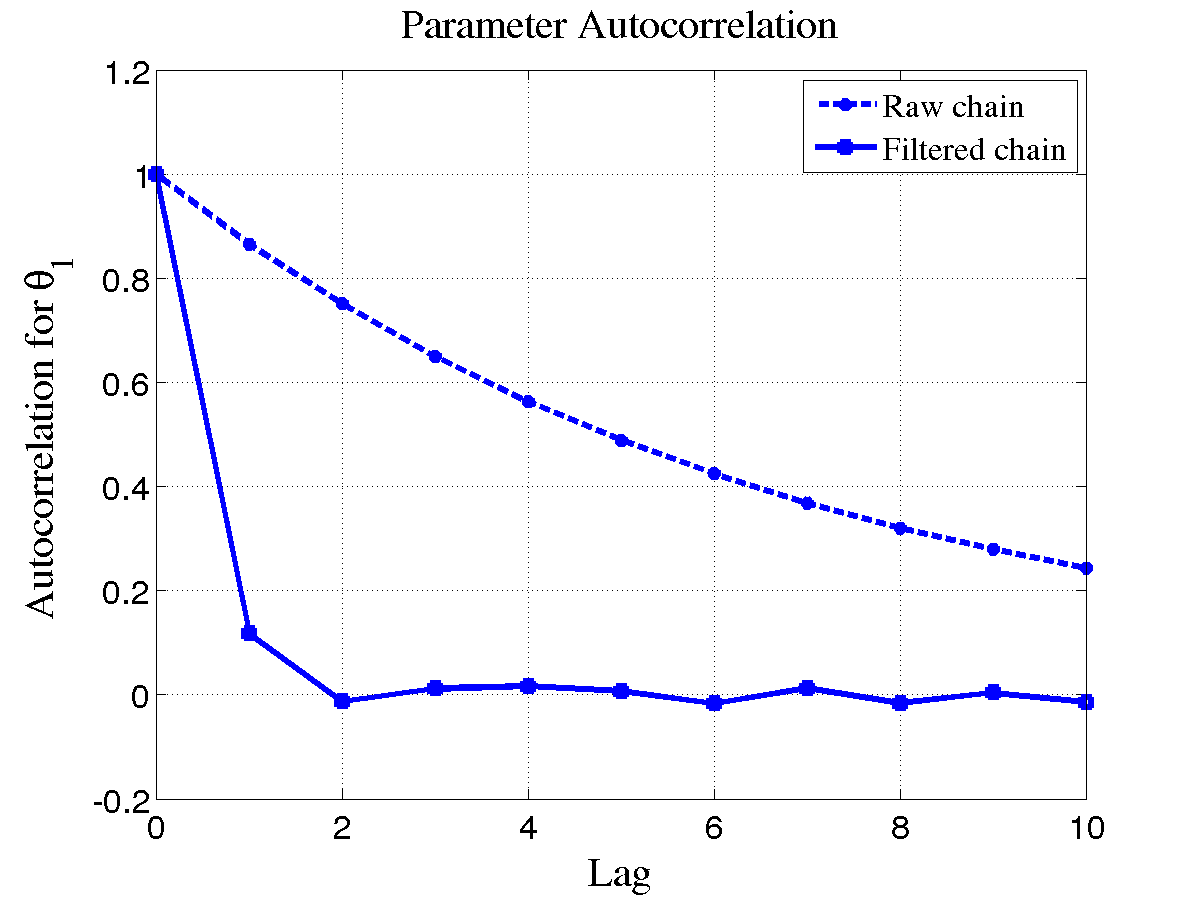
\includegraphics[scale=0.35]{figs/simple_ip_autocorrelation_raw_filt_theta1.png}}
%\subfloat[$\theta_2$]{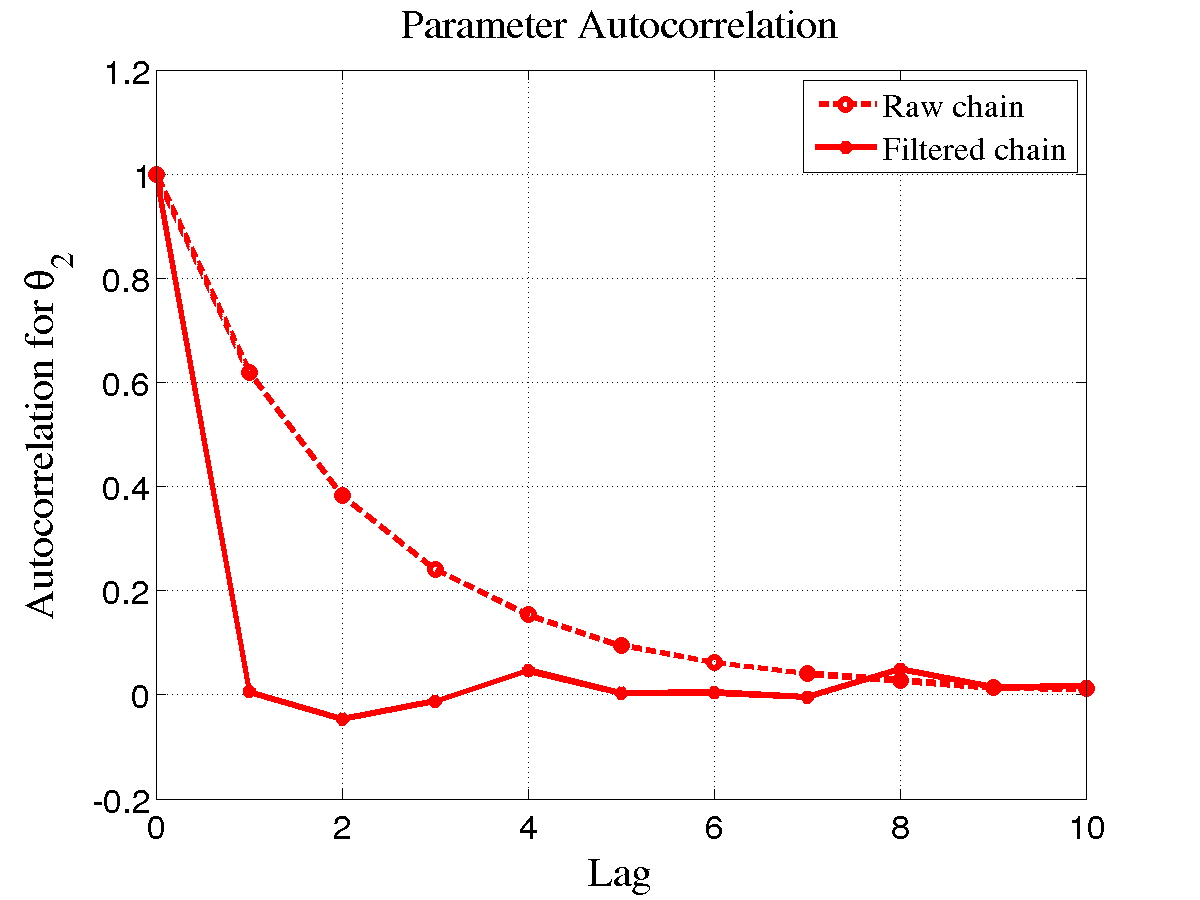
\includegraphics[scale=0.35]{figs/simple_ip_autocorrelation_raw_filt_theta2.png}}
\subfloat{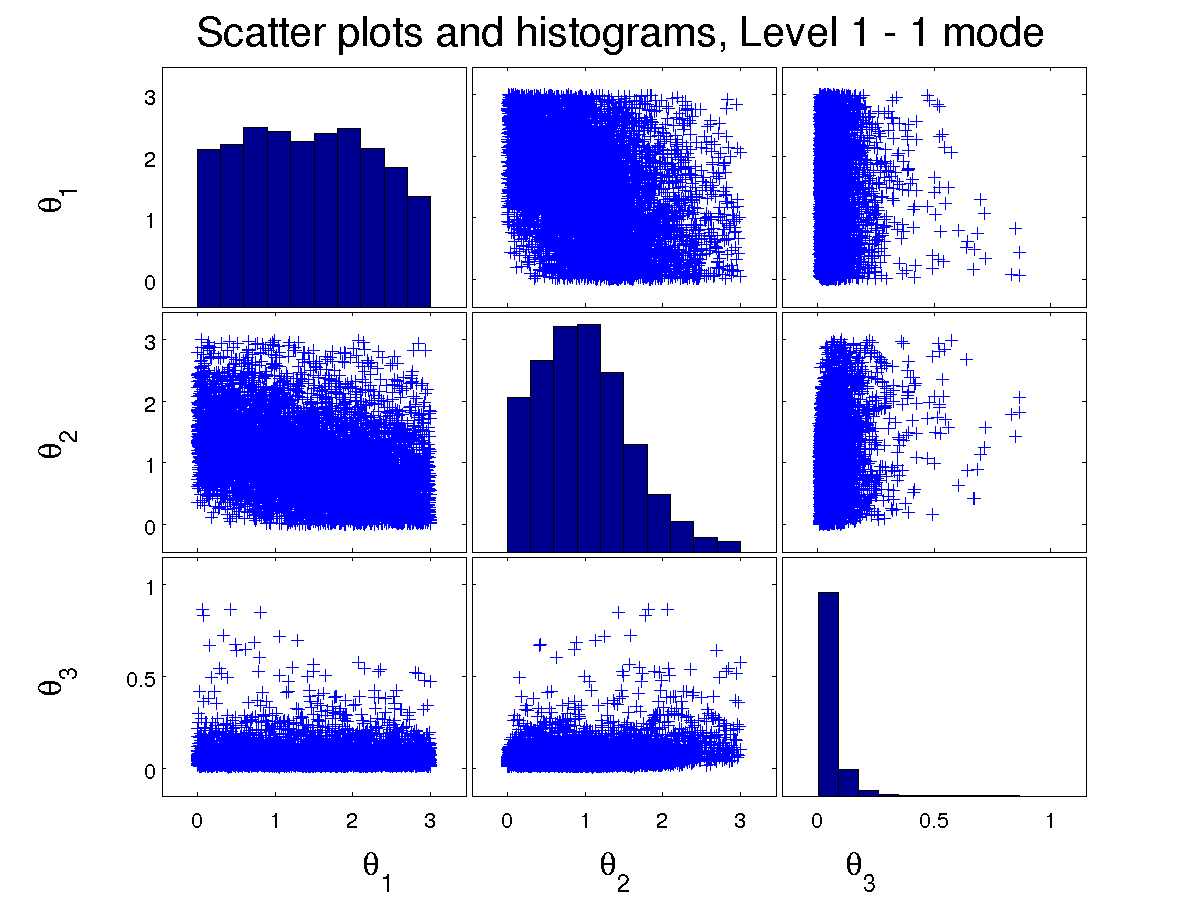
\includegraphics[scale=0.3]{figs/modal_1_mode_level_1.png}}
\subfloat{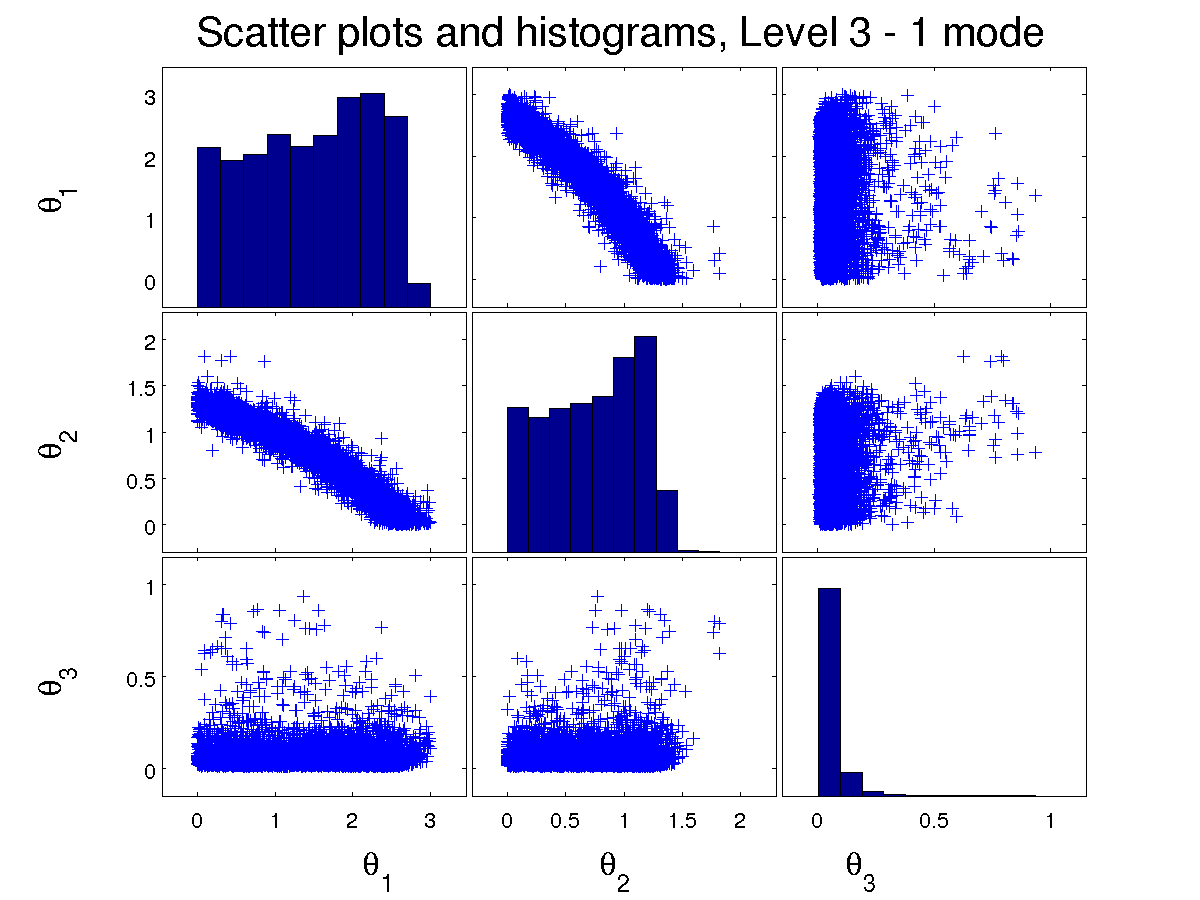
\includegraphics[scale=0.3]{figs/modal_1_mode_level_3.png}}\\
\subfloat{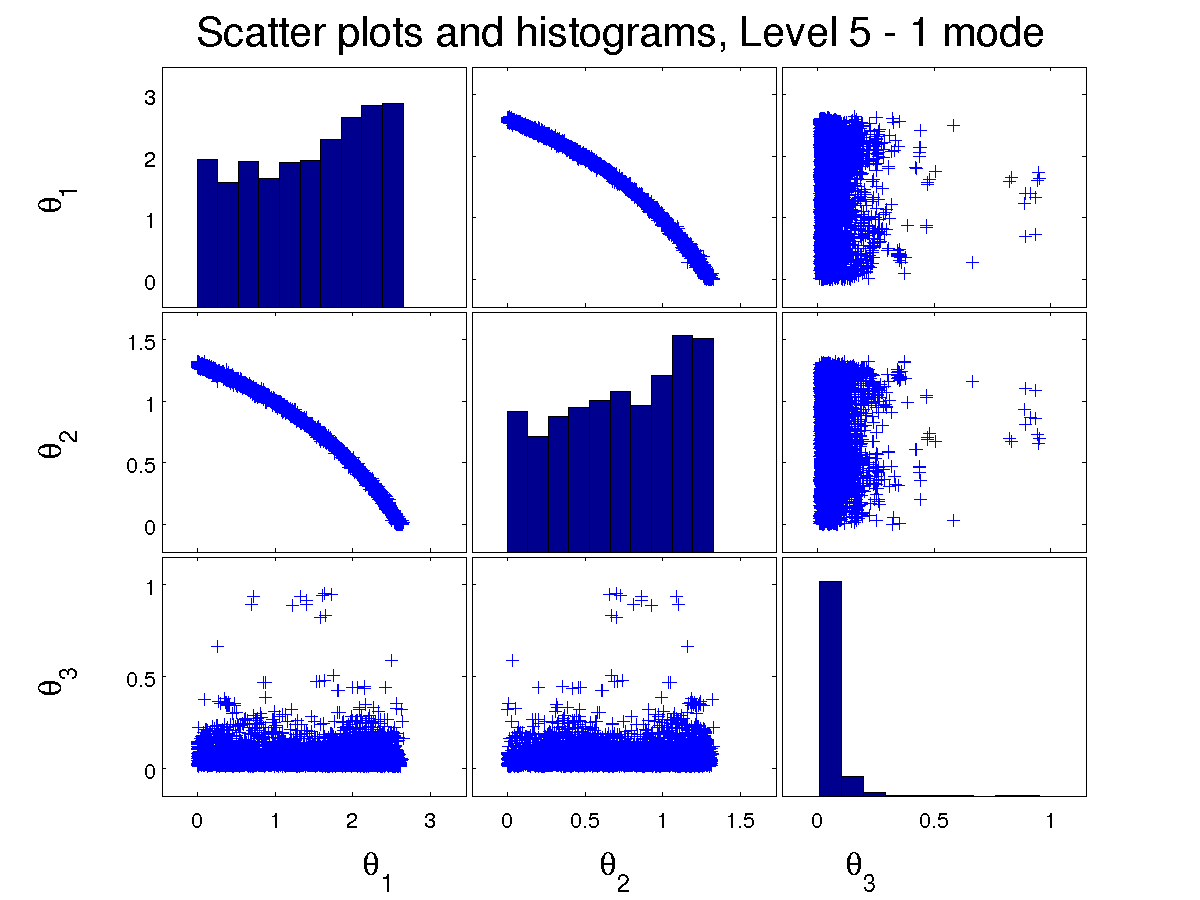
\includegraphics[scale=0.3]{figs/modal_1_mode_level_5.png}}
\subfloat{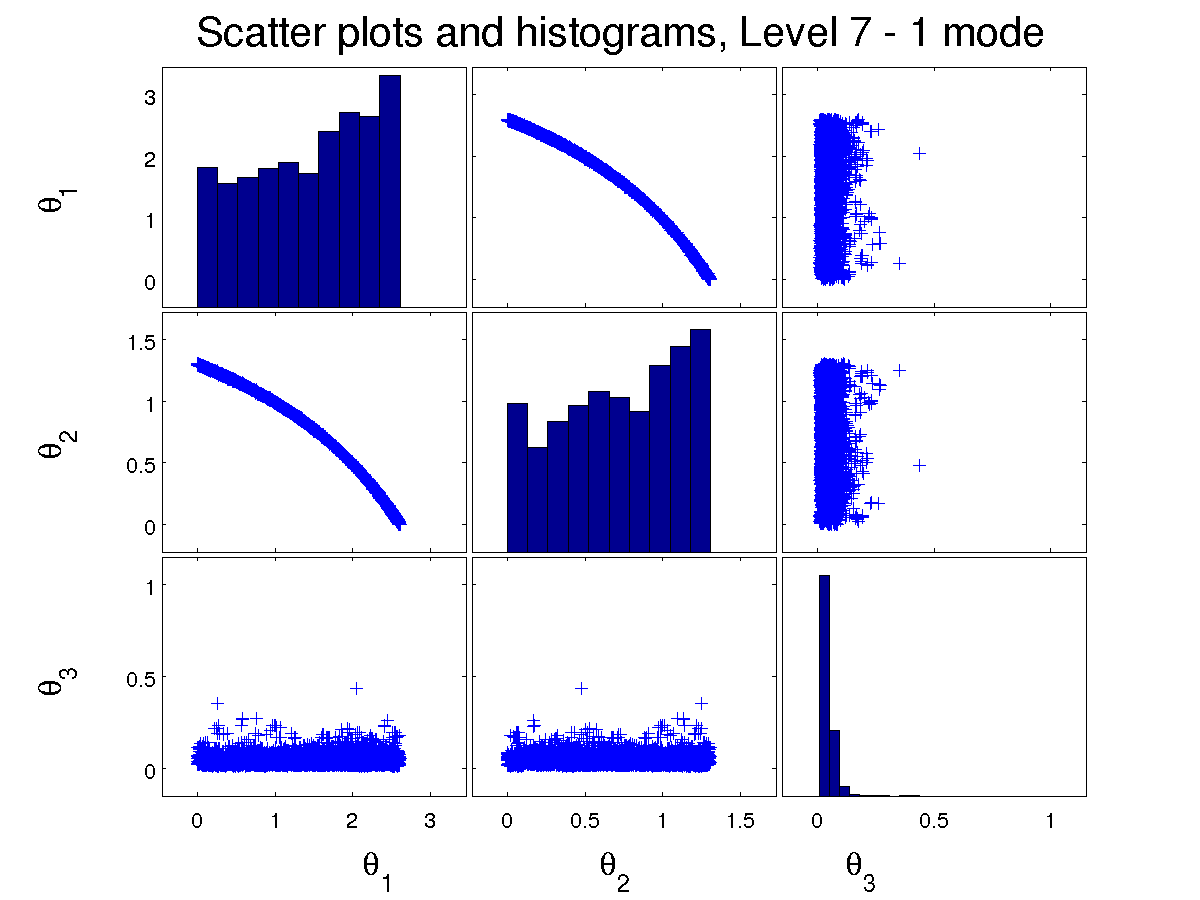
\includegraphics[scale=0.3]{figs/modal_1_mode_level_7.png}}
\vspace{-10pt}
\caption{Scatter plots for $\theta_1$, $\theta_2$ and $\theta_3=\sigma^2$, levels 1, 3, 5 and 7 (last). One mode distribution.}
\label{fig:modal_scatter_1mode}
\end{figure}

\begin{figure}[htpb]
\centering
%\subfloat[$\theta_1$]{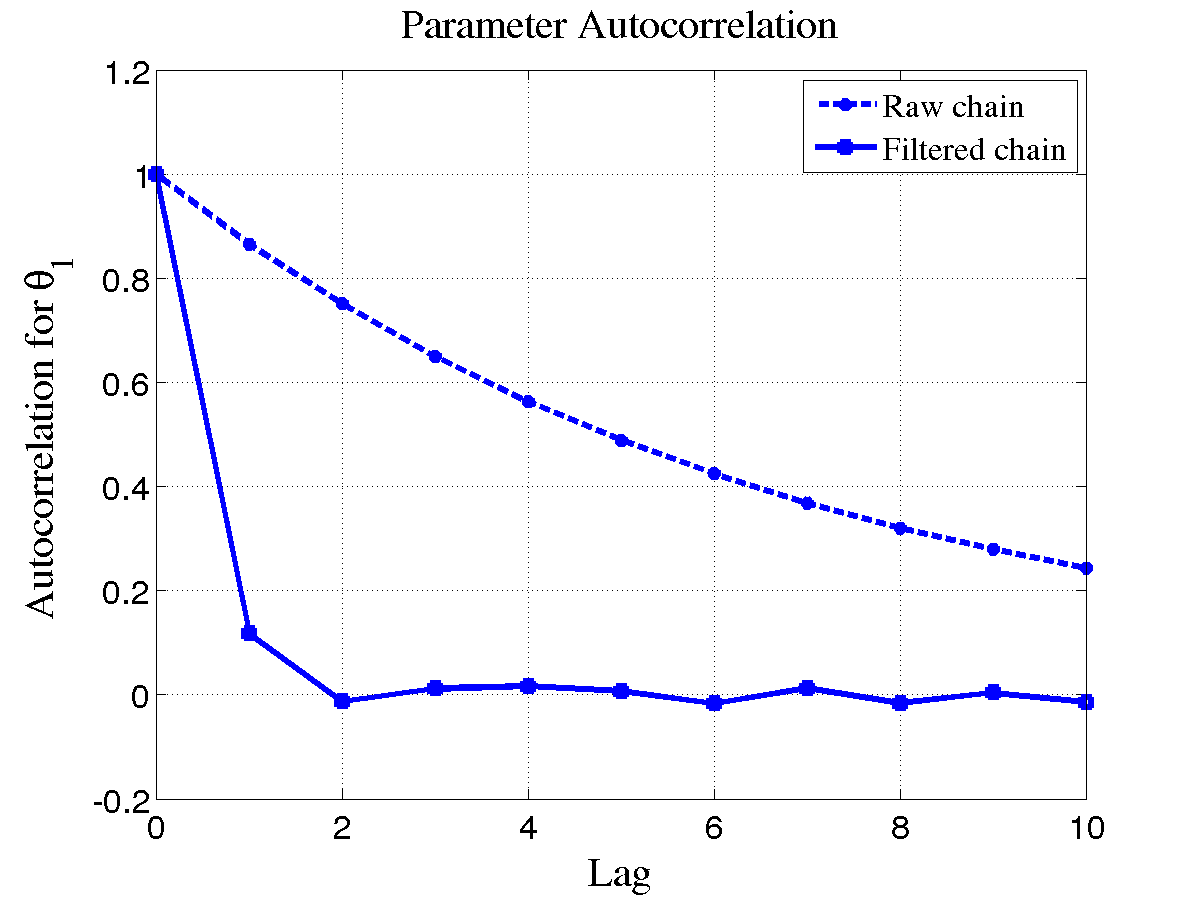
\includegraphics[scale=0.35]{figs/simple_ip_autocorrelation_raw_filt_theta1.png}}
%\subfloat[$\theta_2$]{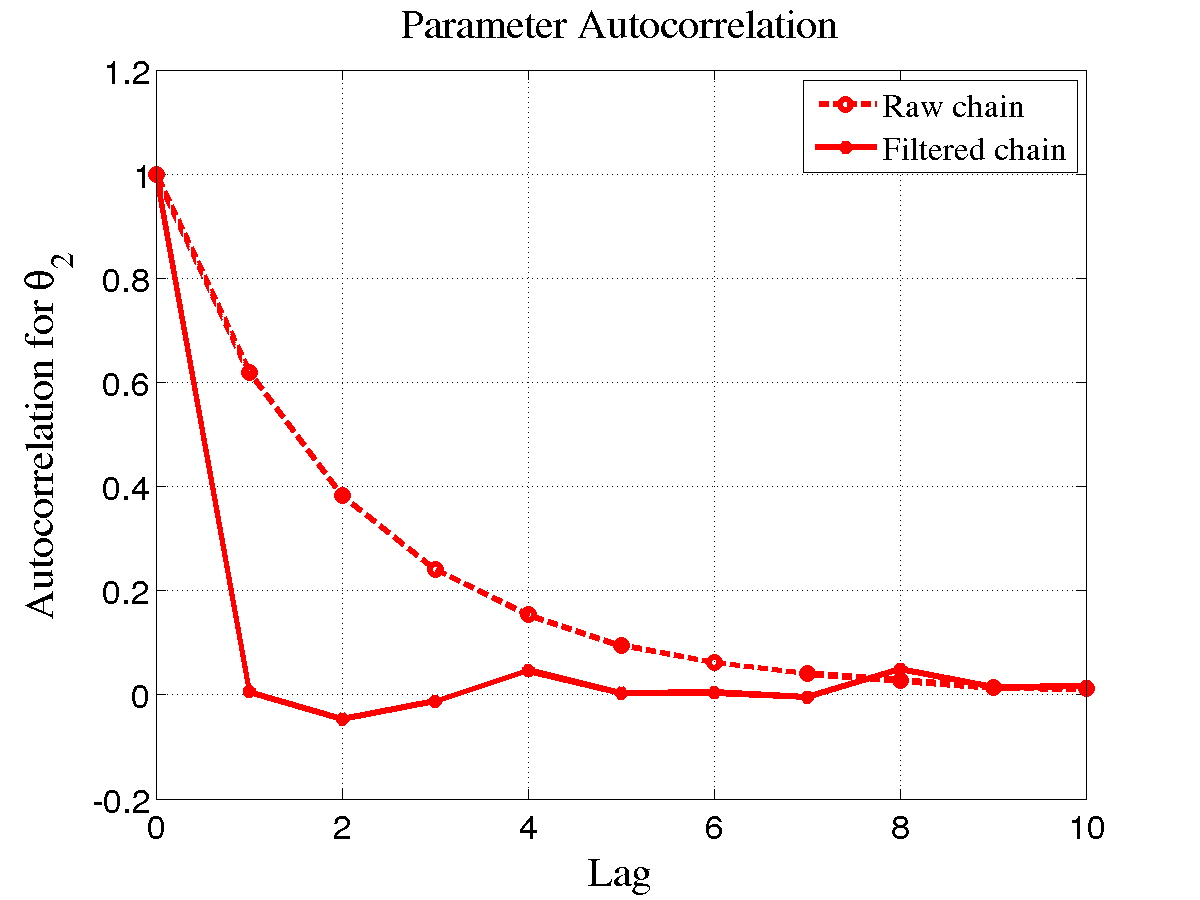
\includegraphics[scale=0.35]{figs/simple_ip_autocorrelation_raw_filt_theta2.png}}
\subfloat{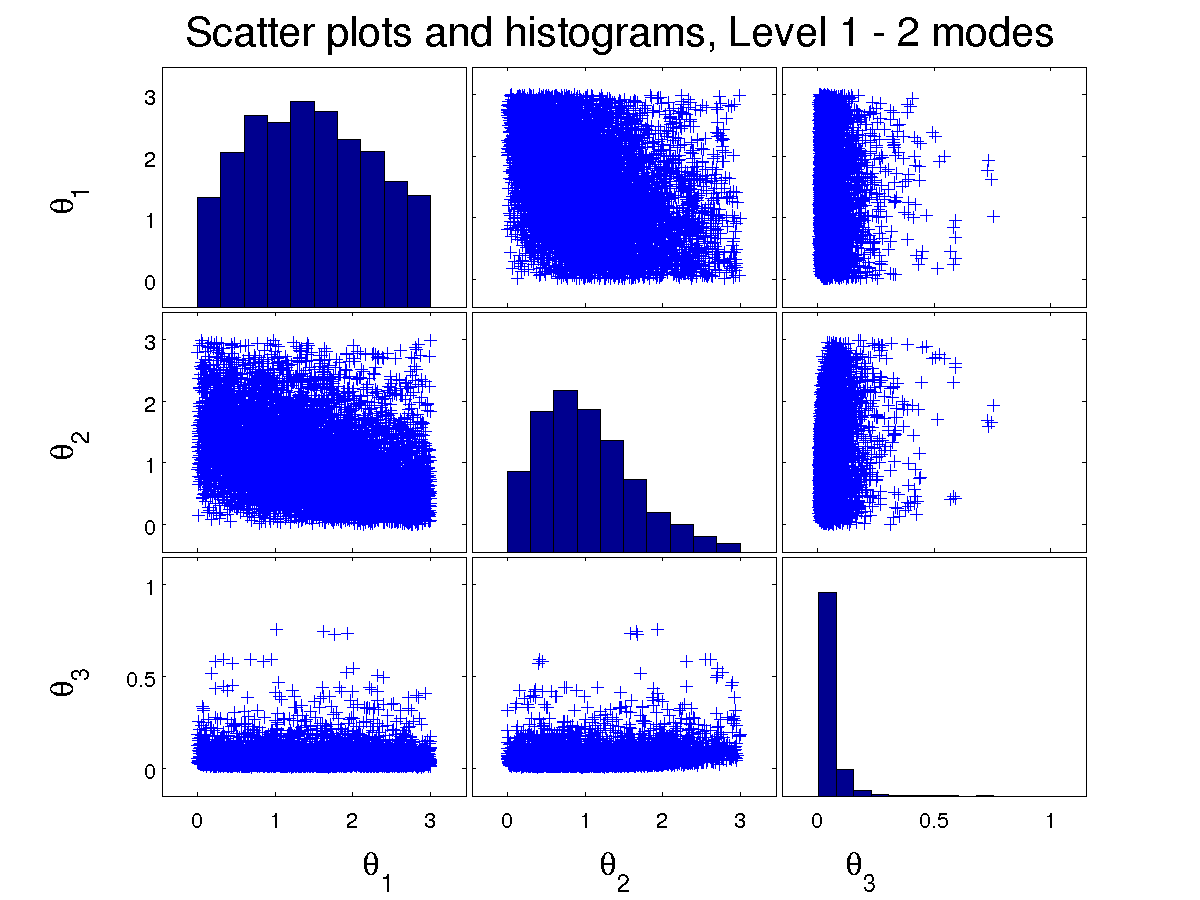
\includegraphics[scale=0.3]{figs/modal_2_modes_level_1.png}}
\subfloat{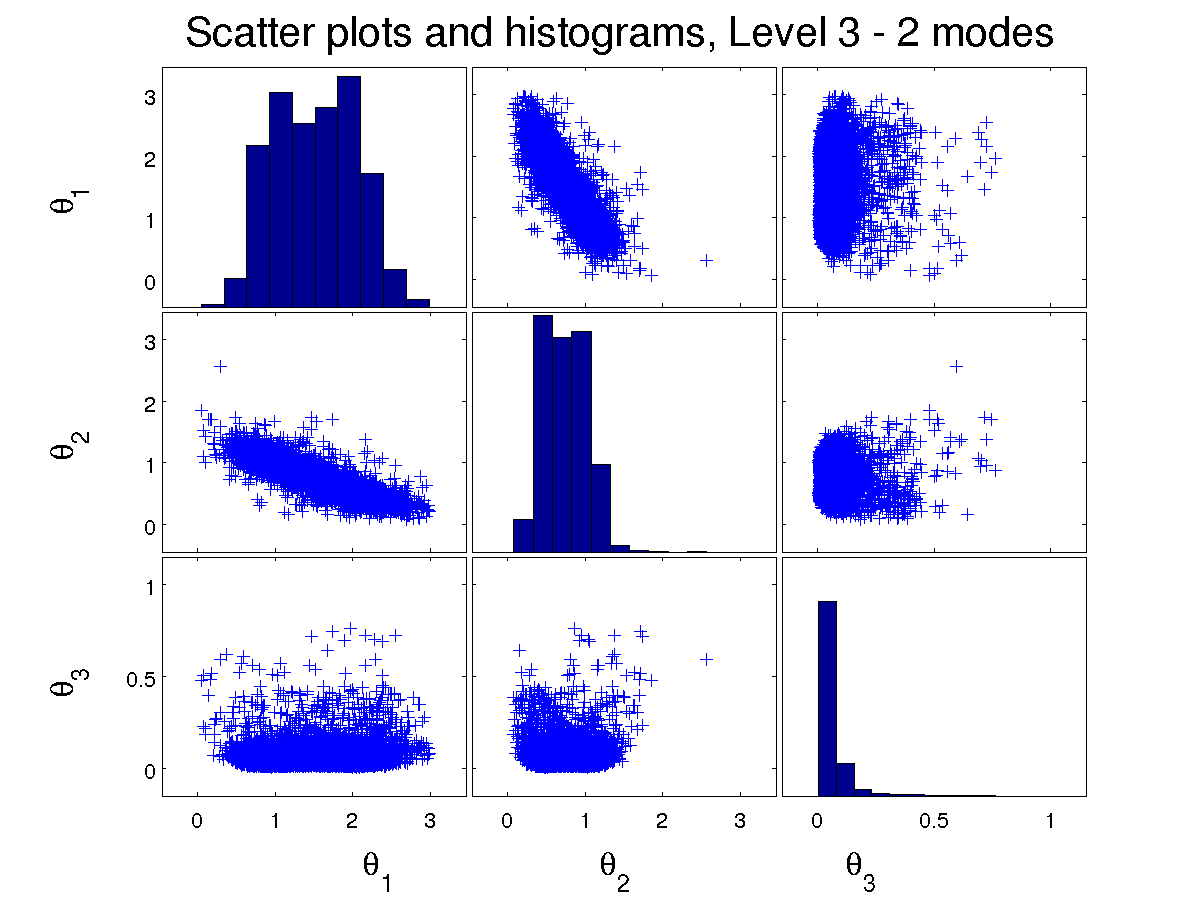
\includegraphics[scale=0.3]{figs/modal_2_modes_level_3.png}}\\
\subfloat{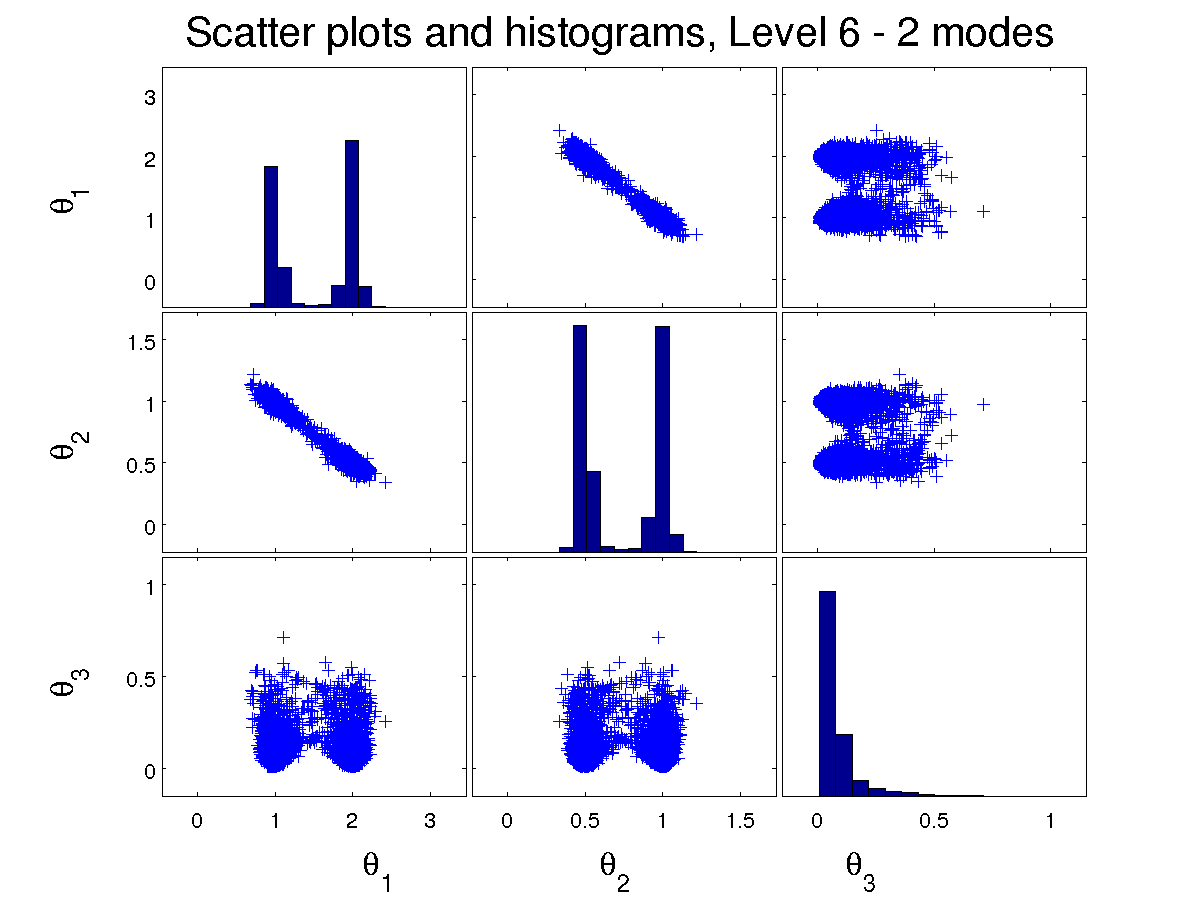
\includegraphics[scale=0.3]{figs/modal_2_modes_level_6.png}}
\subfloat{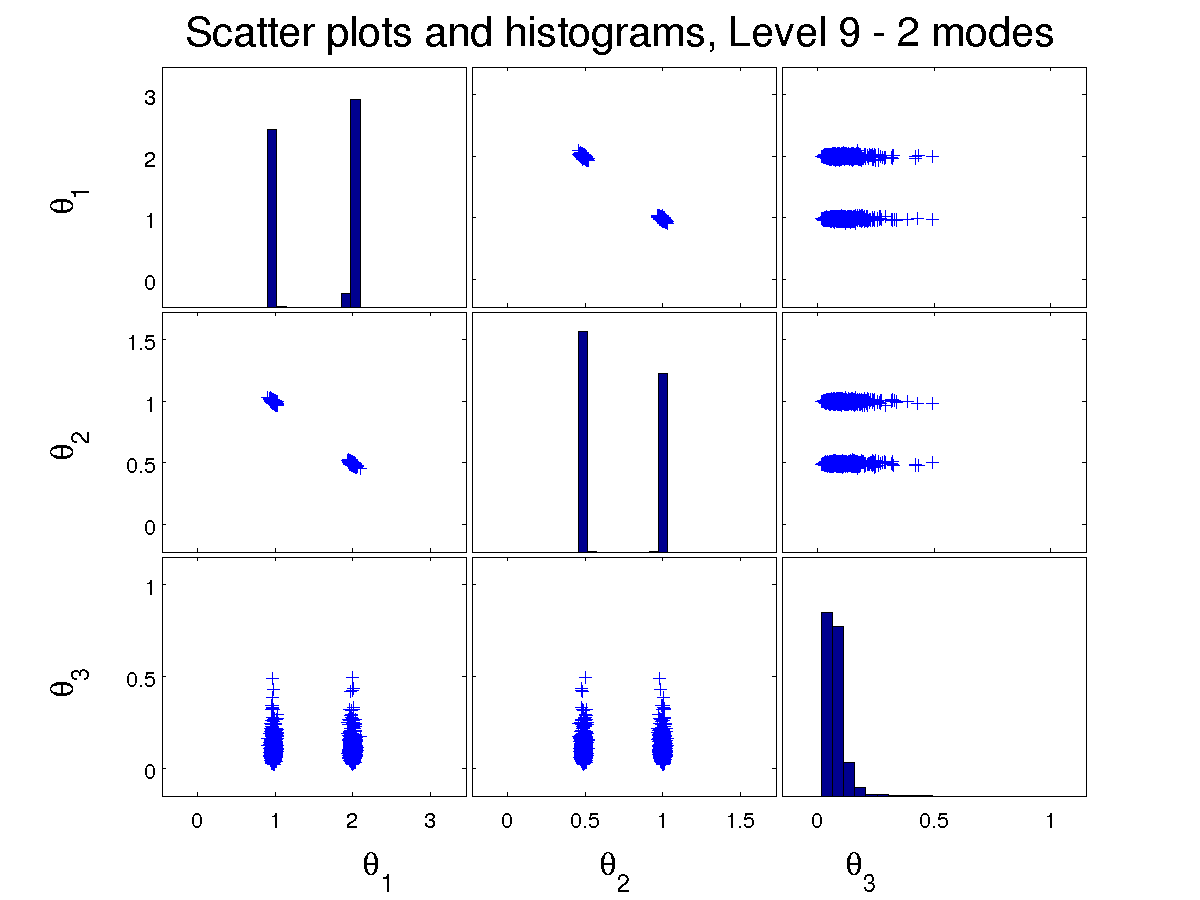
\includegraphics[scale=0.3]{figs/modal_2_modes_level_9.png}}
\vspace{-10pt}
\caption{Scatter plots for $\theta_1$, $\theta_2$ and $\theta_3=\sigma^2$, levels 1, 3, 6 and 9 (last). Two-mode distribution.}
\label{fig:modal_scatter_2modes}
\end{figure}

\subsubsection{KDE Plots}

Figures \ref{fig:modal_kde_1mode} and \ref{fig:modal_kde_2modes} present the KDE plots of the parameters $\theta_1$, $\theta_2$, $\theta_3$ and target PDF in both cases: one-mode and two-modes distribution. 



\begin{figure}[hptb]
\centering
\subfloat{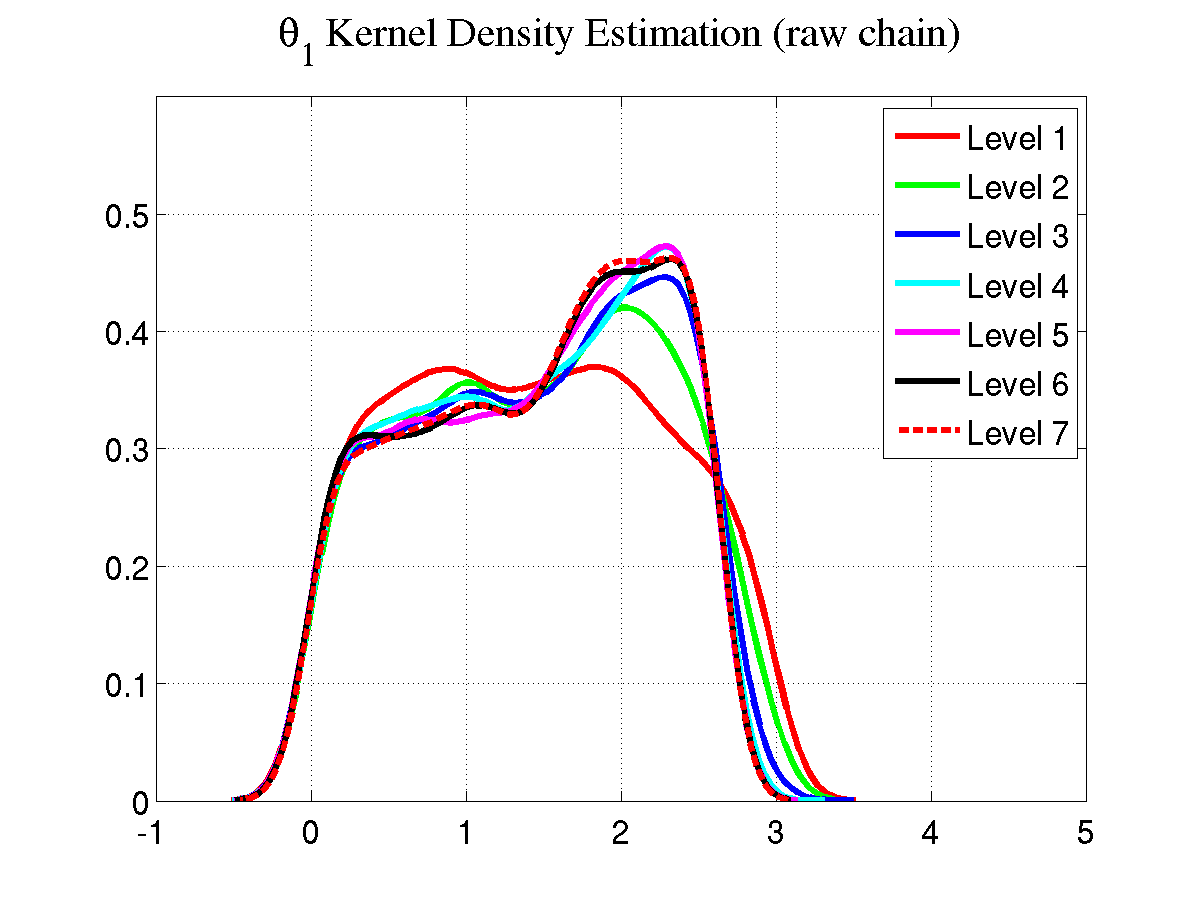
\includegraphics[scale=0.3]{figs/modal_1_mode_kde_theta1.png}}
\subfloat{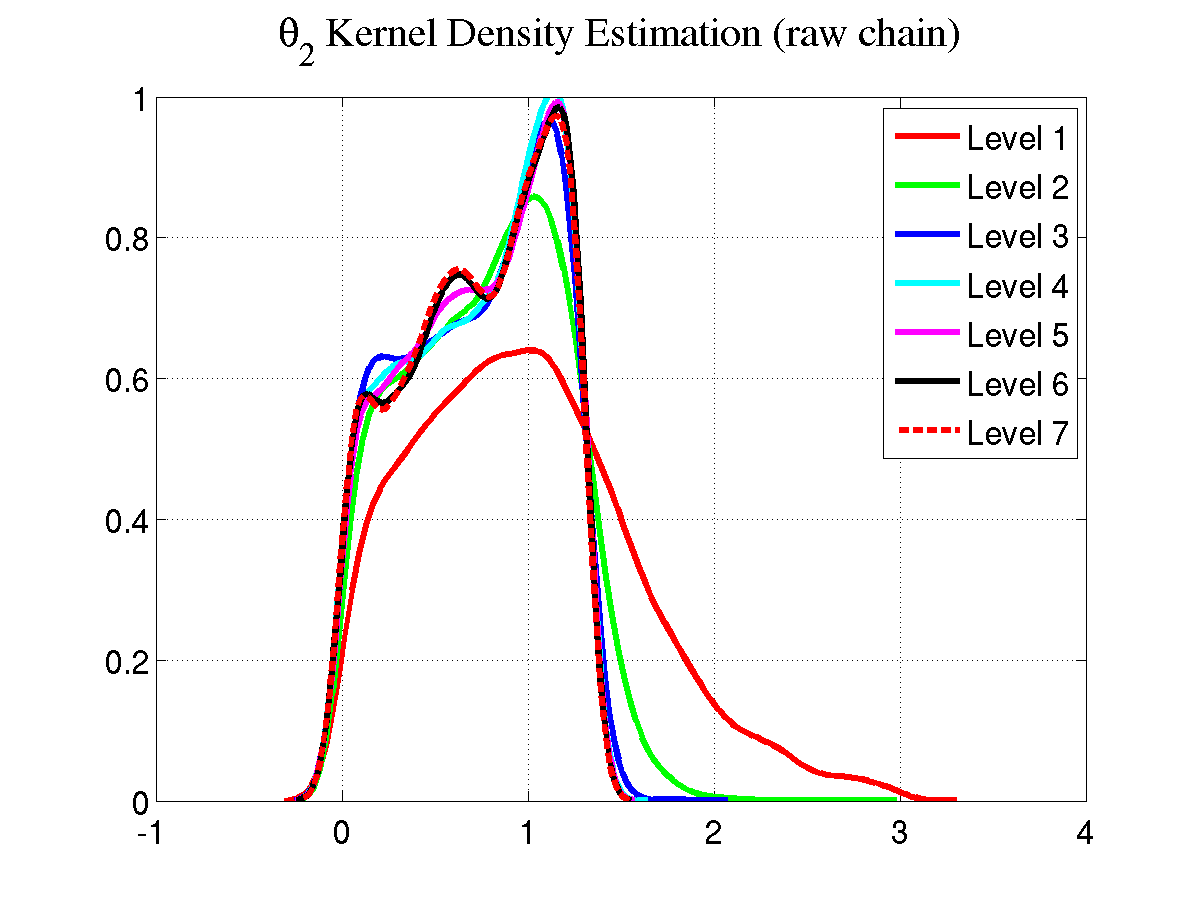
\includegraphics[scale=0.3]{figs/modal_1_mode_kde_theta2.png}}\\
\subfloat{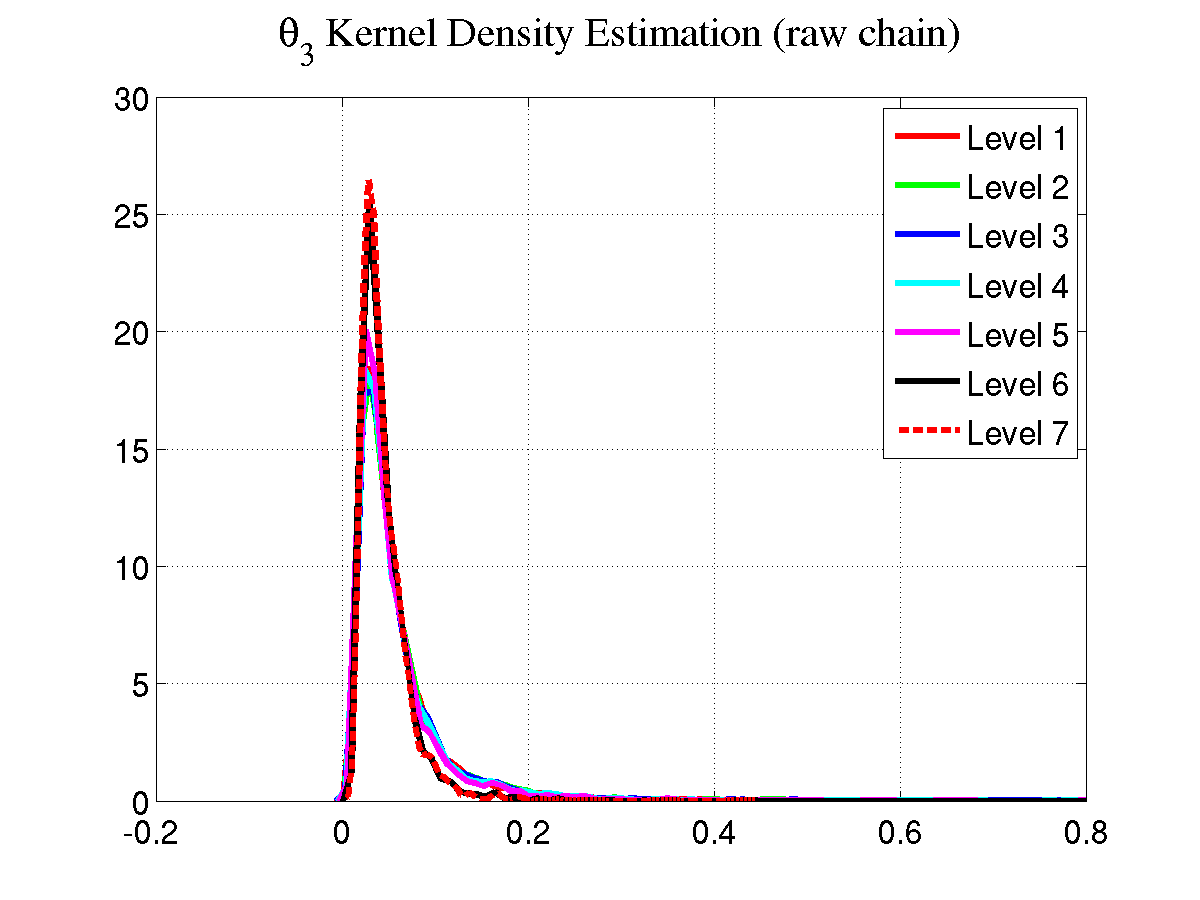
\includegraphics[scale=0.3]{figs/modal_1_mode_kde_theta3.png}}
\subfloat{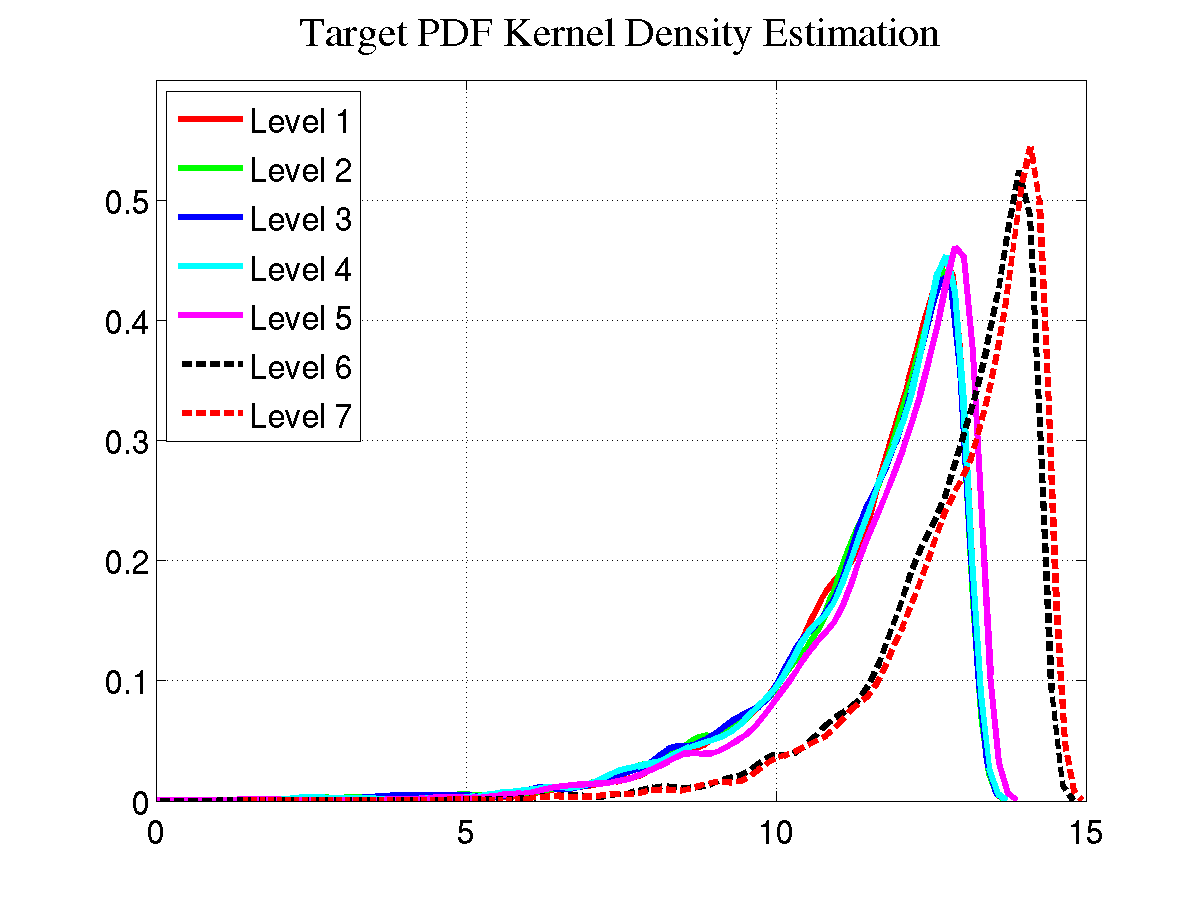
\includegraphics[scale=0.3]{figs/modal_1_mode_kde_target.png}}
\vspace{-10pt}
\caption{KDE plots for $\theta_1$, $\theta_2$, $\theta_3=\sigma^2$, and the target PDF. One mode distribution.}
\label{fig:modal_kde_1mode}
\end{figure}

\begin{figure}[hptb]
\centering
\subfloat{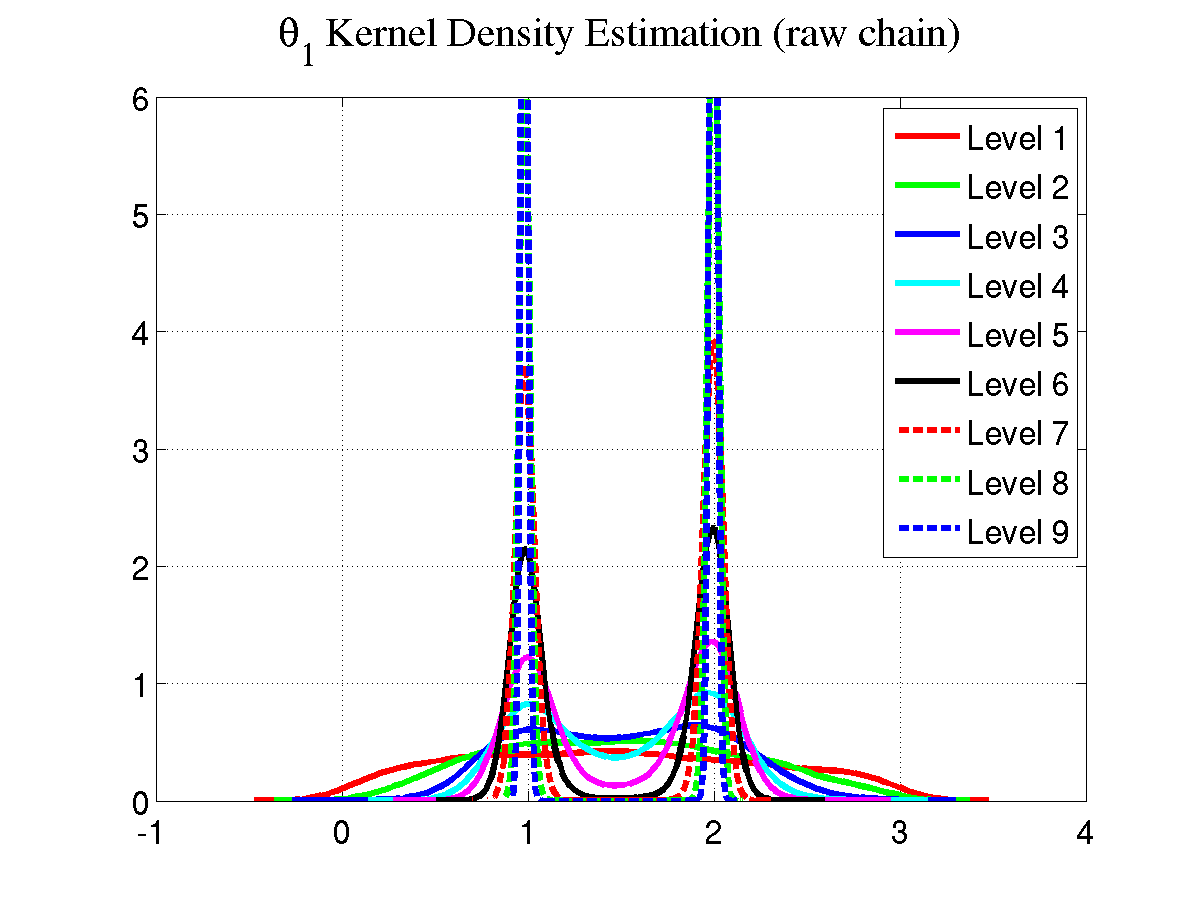
\includegraphics[scale=0.3]{figs/modal_2_modes_kde_theta1.png}}
\subfloat{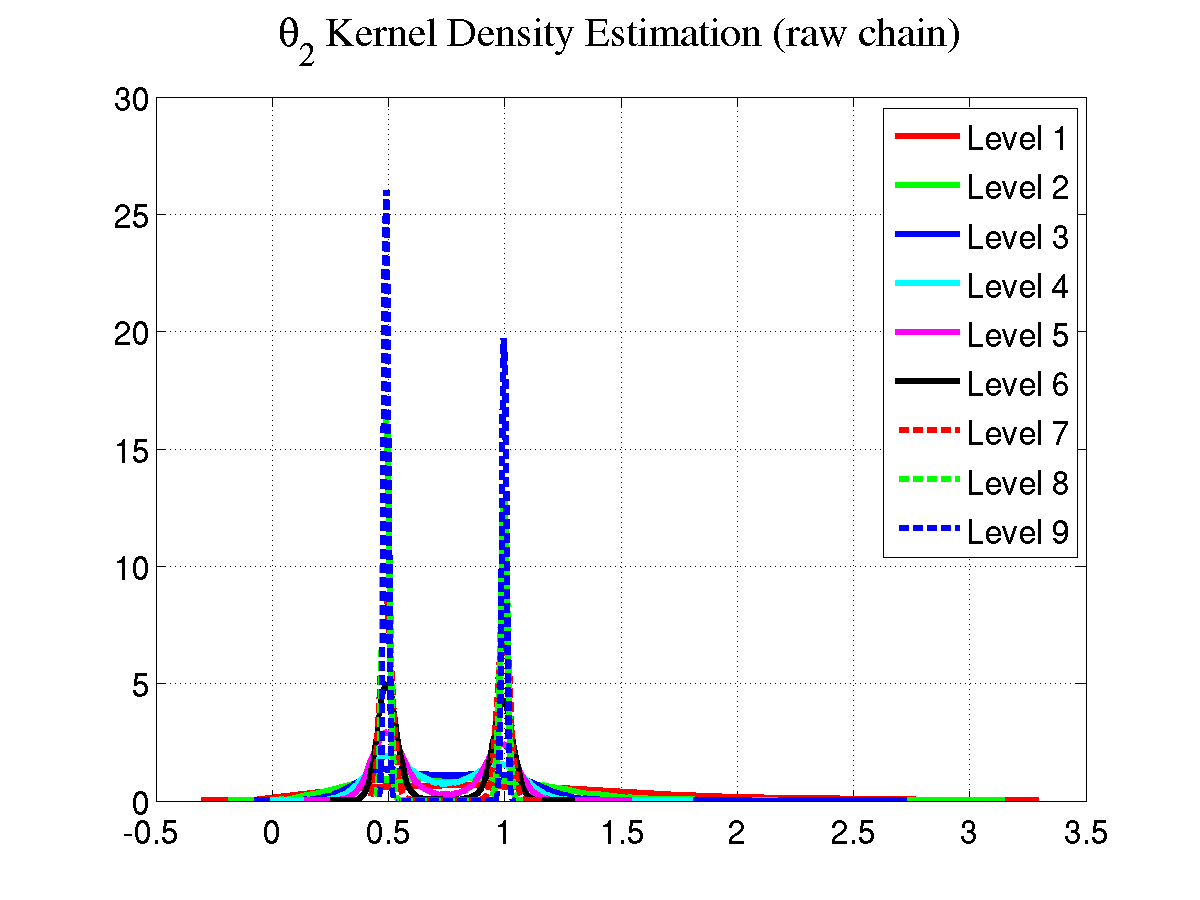
\includegraphics[scale=0.3]{figs/modal_2_modes_kde_theta2.png}}\\
\subfloat{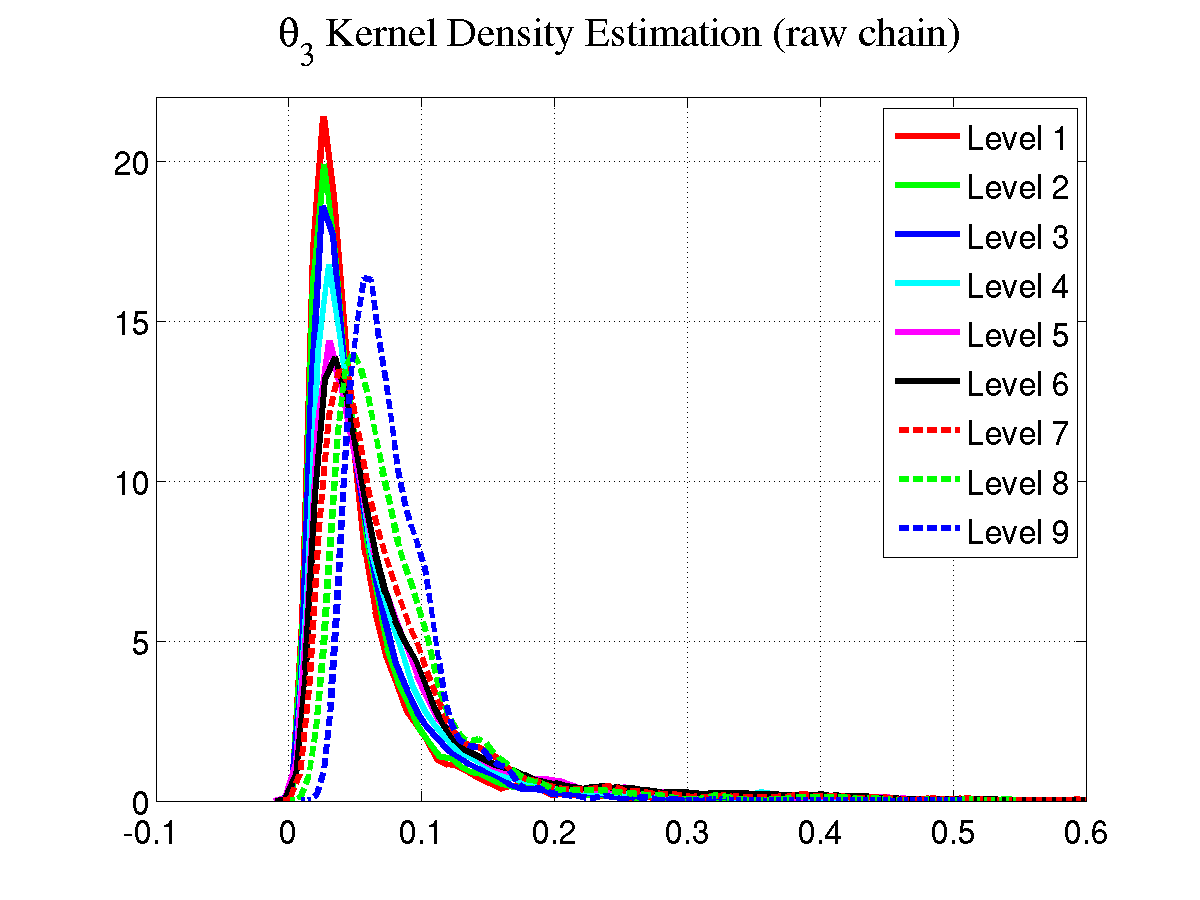
\includegraphics[scale=0.3]{figs/modal_2_modes_kde_theta3.png}}
\subfloat{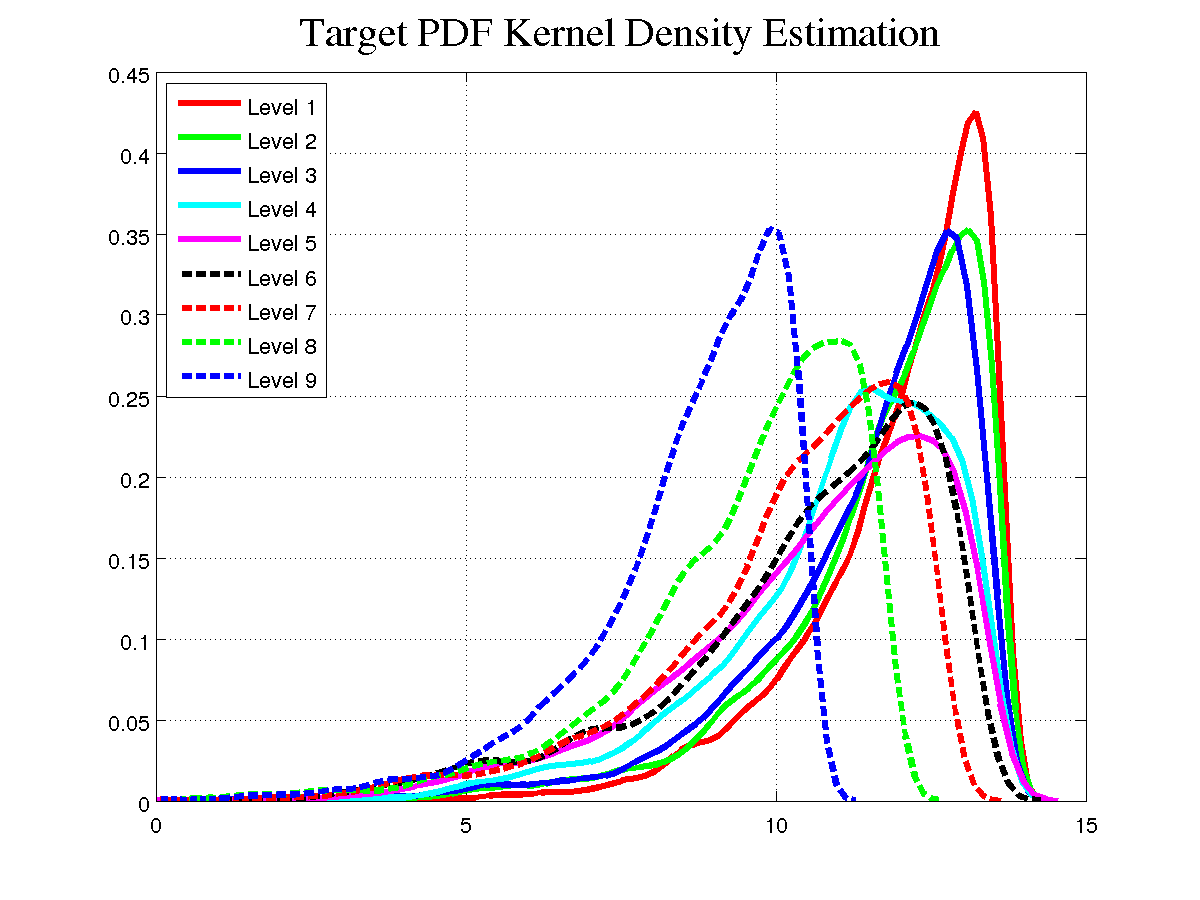
\includegraphics[scale=0.3]{figs/modal_2_modes_kde_target.png}}
\vspace{-10pt}
\caption{KDE plots for $\theta_1$, $\theta_2$, $\theta_3=\sigma^2$, and the target PDF. Two-mode distribution.}
\label{fig:modal_kde_2modes}
\end{figure}


\subsubsection{Autocorrelation Plots}

Figures \ref{fig:modal_autocorr_1mode} and \ref{fig:modal_autocorr_2modes} present the autocorrelation of the parameters $\theta_1$, $\theta_2$ and $\theta_3$ in both cases: one-mode and two-modes distribution.

\begin{figure}[htpb]
\centering
\subfloat{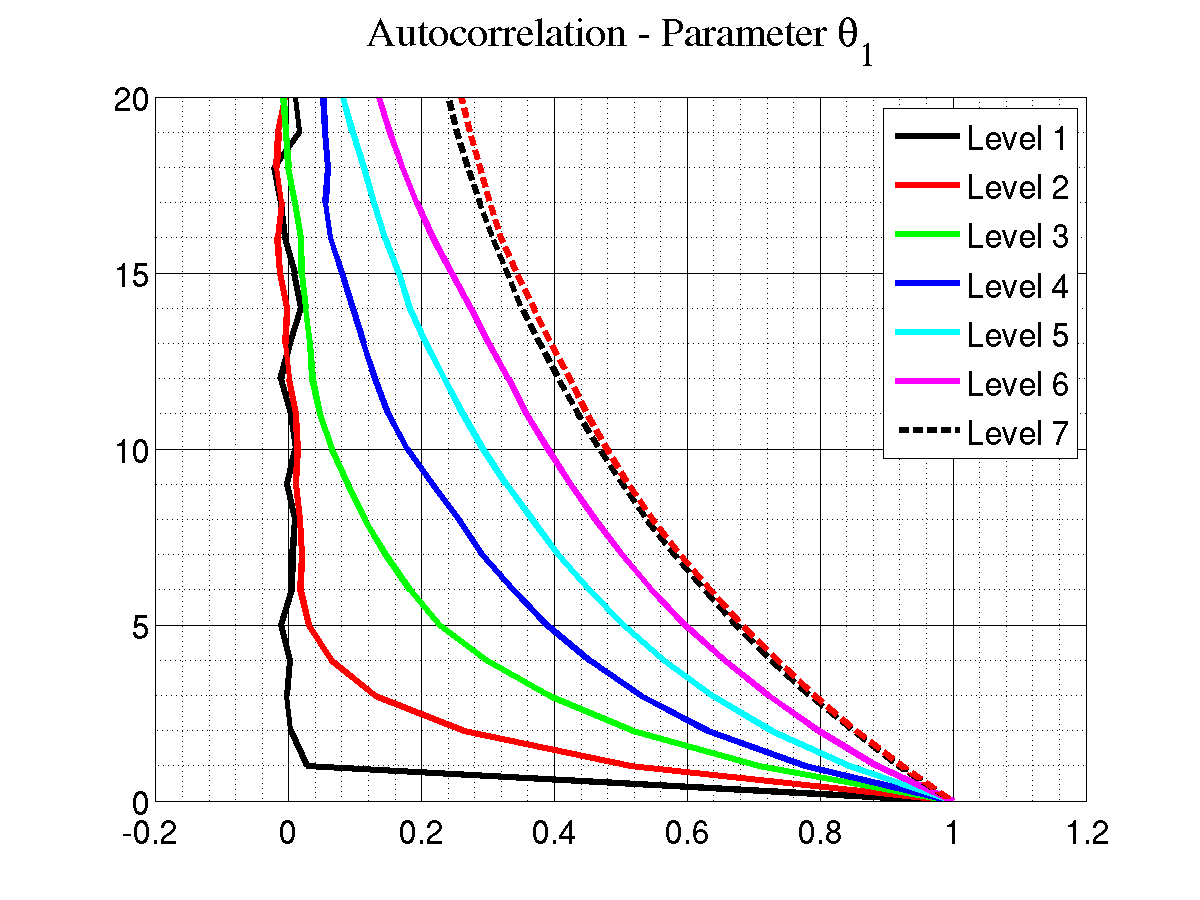
\includegraphics[scale=0.25]{figs/modal_1_mode_autocorrelation_theta1.png}}
\subfloat{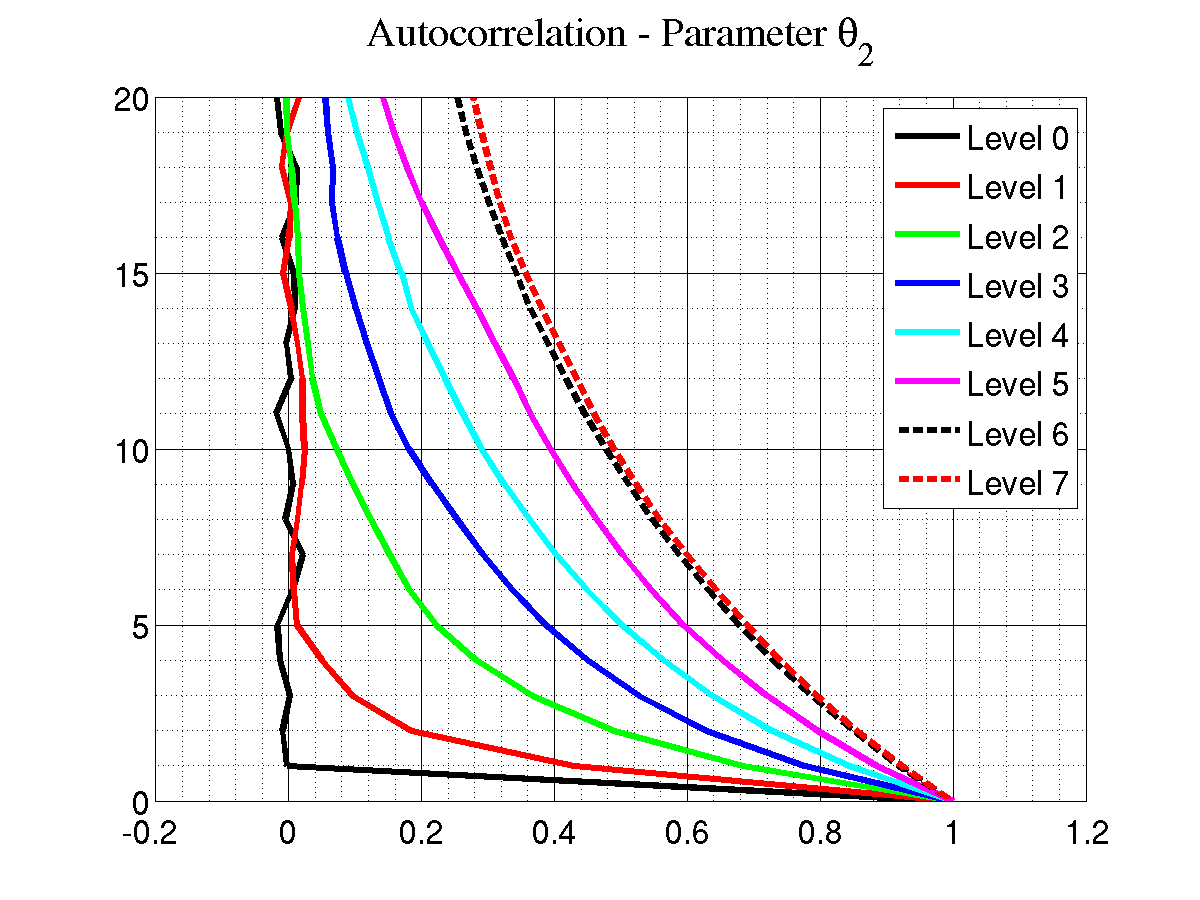
\includegraphics[scale=0.25]{figs/modal_1_mode_autocorrelation_theta2.png}}
\subfloat{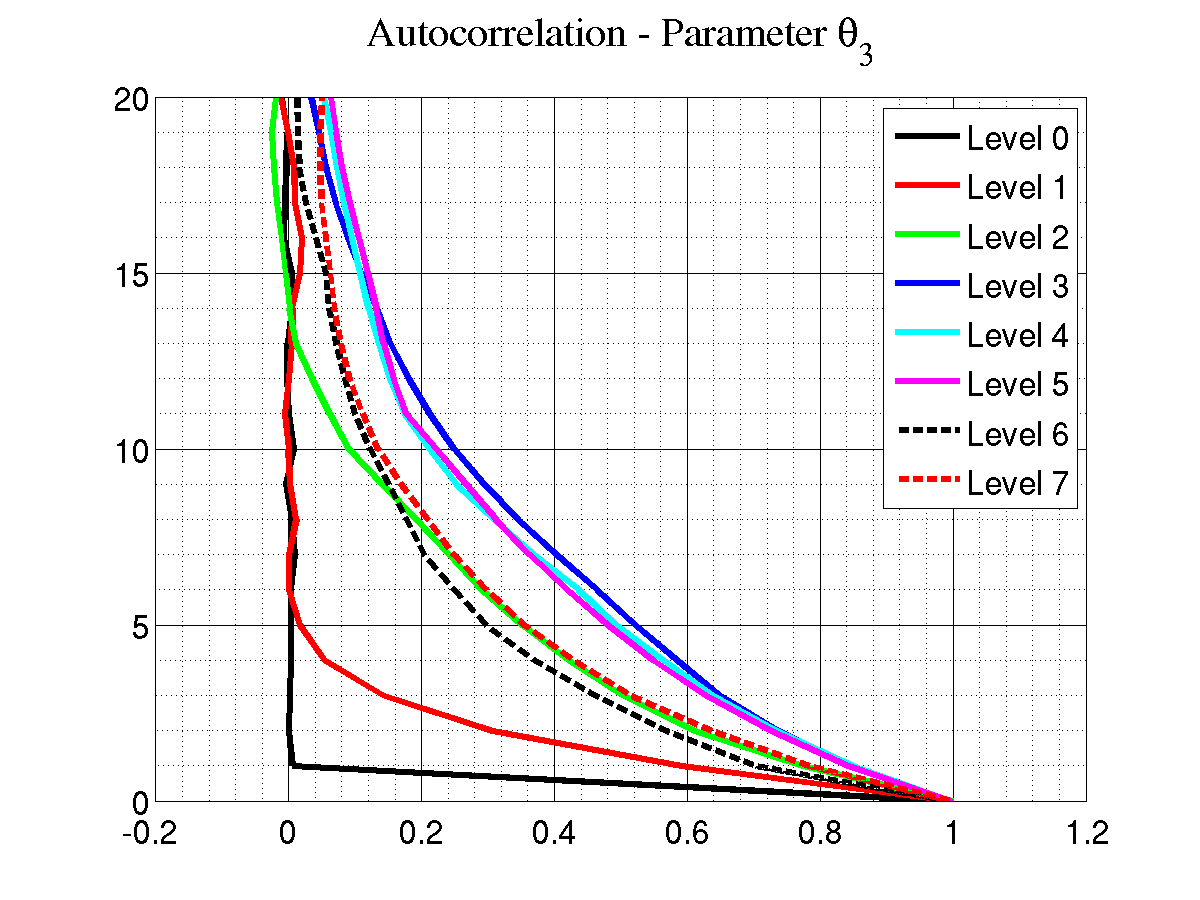
\includegraphics[scale=0.25]{figs/modal_1_mode_autocorrelation_theta3.png}}
\vspace{-10pt}
\caption{Autocorrelation plots for $\theta_1$, $\theta_2$ and $\theta_3=\sigma^2$. One-mode distribution.}
\label{fig:modal_autocorr_1mode}
\end{figure}

\begin{figure}[htpb]
\centering
\subfloat{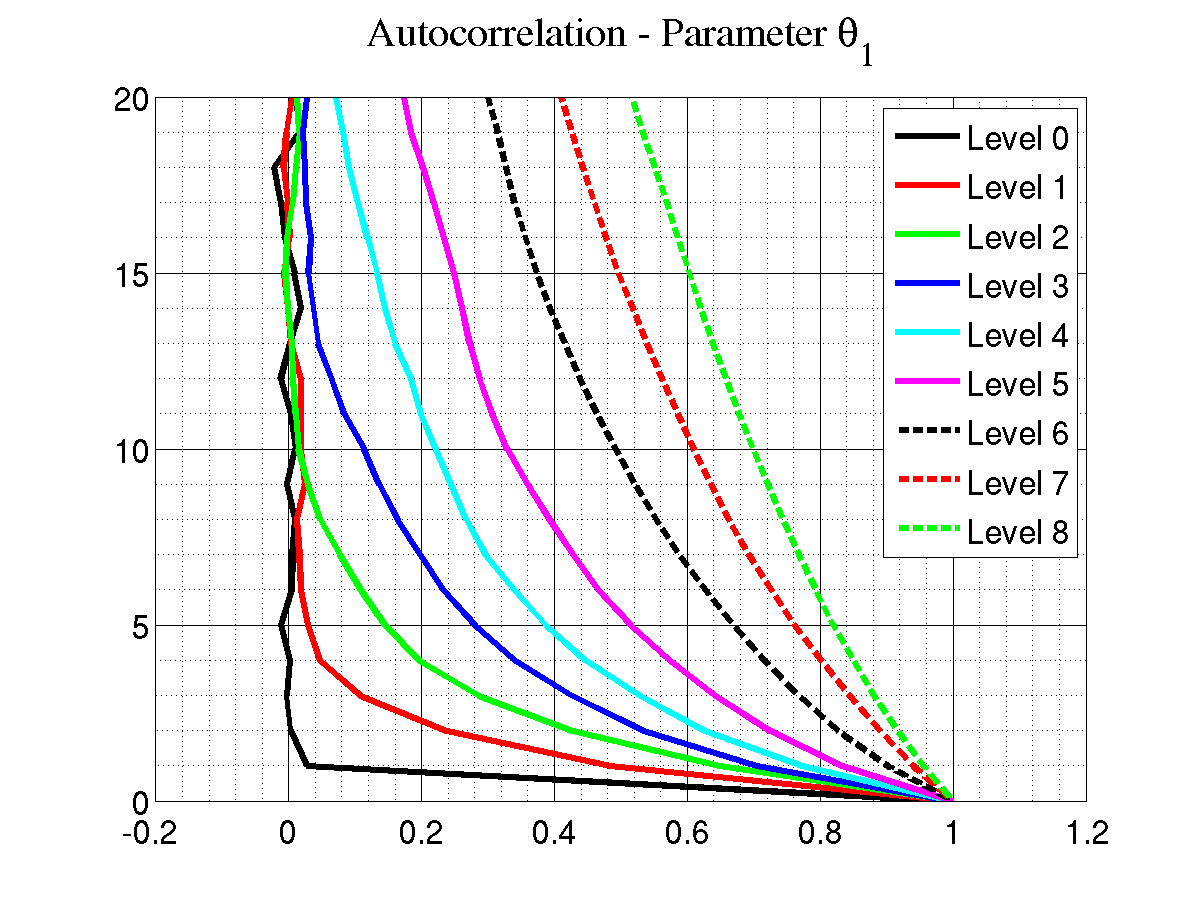
\includegraphics[scale=0.25]{figs/modal_2_modes_autocorrelation_theta1.png}}
\subfloat{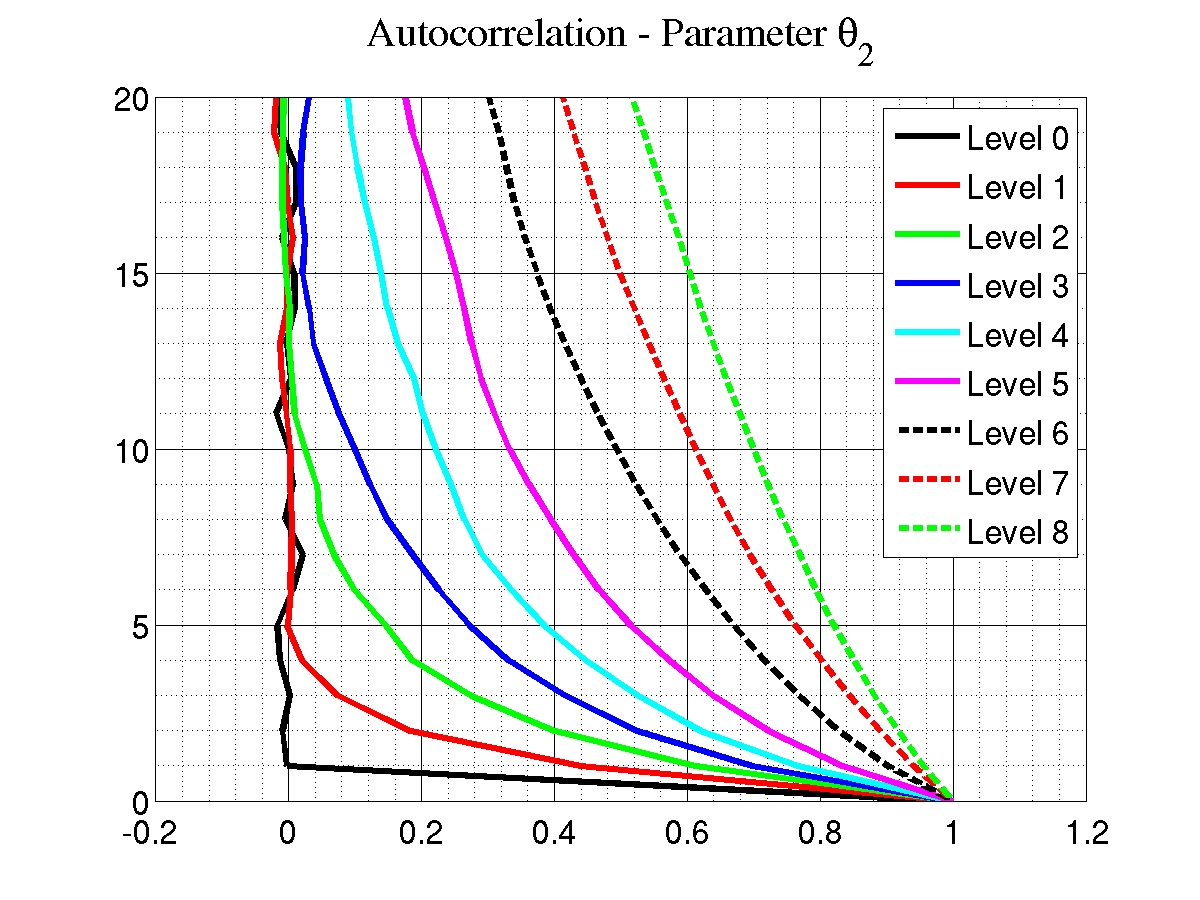
\includegraphics[scale=0.25]{figs/modal_2_modes_autocorrelation_theta2.png}}
\subfloat{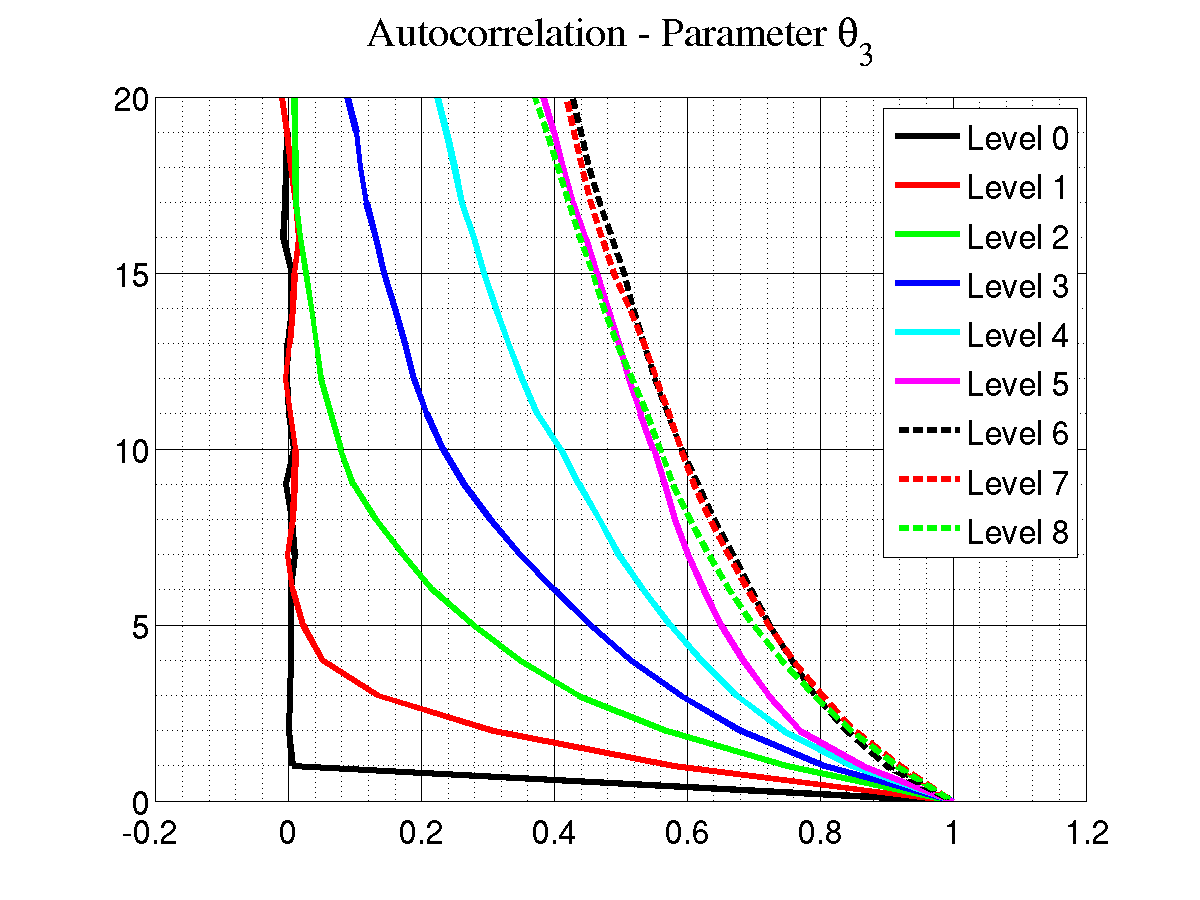
\includegraphics[scale=0.25]{figs/modal_2_modes_autocorrelation_theta3.png}}
\vspace{-10pt}
\caption{Autocorrelation plots for $\theta_1$, $\theta_2$ and $\theta_3=\sigma^2$. Two-mode distribution.}
\label{fig:modal_autocorr_2modes}
\end{figure}